\chapter{Implementasi dan Pengujian}
\label{chap:implementation}
Pada bagian ini akan dijelaskan mengenai lingkungan implementasi perangkat keras maupun perangkat lunak. Serta implementasi program iCalendar Converter beserta tampilan antar muka. Terakhir akan dibahas mengenai pengujian pada perangkat lunak ini.

\section{Lingkungan Implementasi}

\subsection{Lingkungan Perangkat Keras}
Dalam mengembangakan perangkat ini, digunakan spesifikasi perangkat keras sebagai berikut:
\begin{itemize}
	\item \textit{Processor} : Intel Core i7 2.4 Ghz
	\item \textit{Memory} : 8 GB
	\item \textit{Hardisk} : 640 GB
	\item VGA : Nvidia GeForce 540M
	\item \textit{keyboard} dan \textit{mouse standard}
\end{itemize}

\subsection{Lingkungan Perangkat Lunak}
Untuk pengembangan perangkat lunak iCalendar Converter, digunakan spesifikasi sebagai berikut:
\begin{itemize}
	\item \textit{Tools:} Netbeans 8.1
	\item Bahasa Pemograman Java 
	\item Serta library seperti JavaFX, Apache POI, dan iCal4j
	\item Tampilan antarmuka menggunakan SceneBuilder
\end{itemize}

\section{Implementasi Program}
Berikut ini merupakan kode program dari perangkat lunak iCalendarConverter :
\begin{enumerate}
	\item Kode Program untuk menyimpan jadwal
		\begin{figure}[H]
		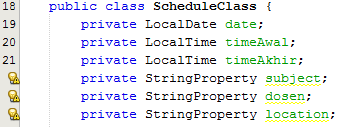
\includegraphics[scale=0.8]{Gambar/scheduleClass}
		\end{figure}
		\begin{figure}[H]
		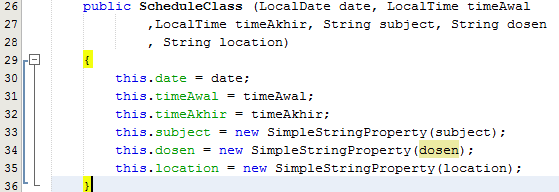
\includegraphics[scale=0.8]{Gambar/scheduleClass5}
		\end{figure}
		\begin{figure}[H]
		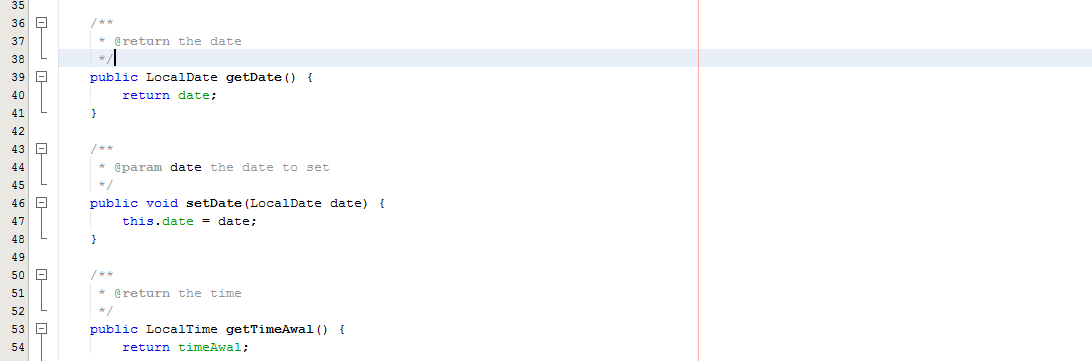
\includegraphics[scale=0.8]{Gambar/scheduleClass1}
		\end{figure}
		\begin{figure}[H]
		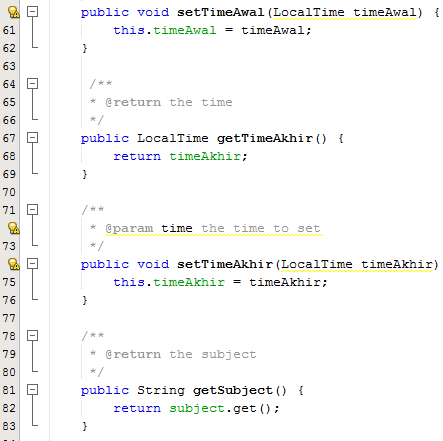
\includegraphics[scale=0.8]{Gambar/scheduleClass2}
		\end{figure}
		\begin{figure}[H]
		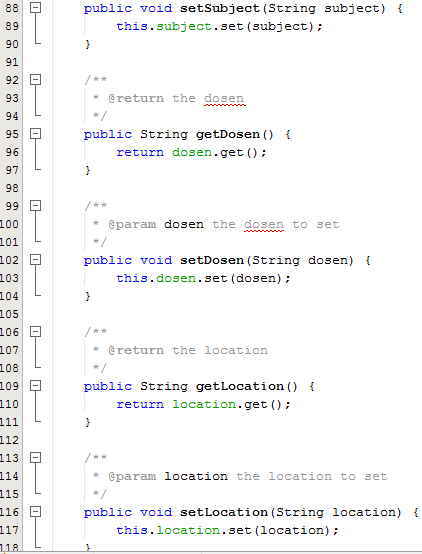
\includegraphics[scale=0.8]{Gambar/scheduleClass3}
		\end{figure}
		\begin{figure}[H]
		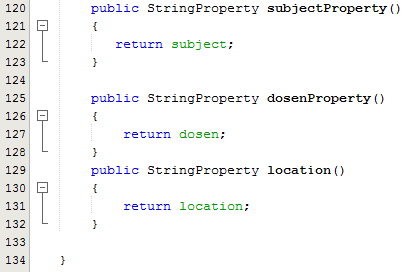
\includegraphics[scale=0.8]{Gambar/scheduleClass4}
		\end{figure}
	\item Kode Program untuk membaca excel dan menampilkannya pada perangkat lunak
		\begin{figure}[H]
		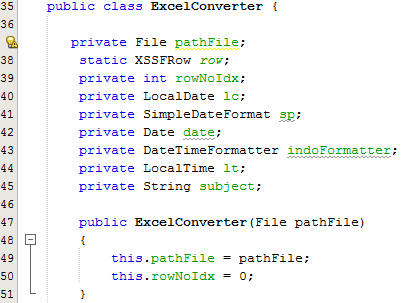
\includegraphics[scale=0.8]{Gambar/excelConverter}
		\end{figure}
		\begin{figure}[H]
		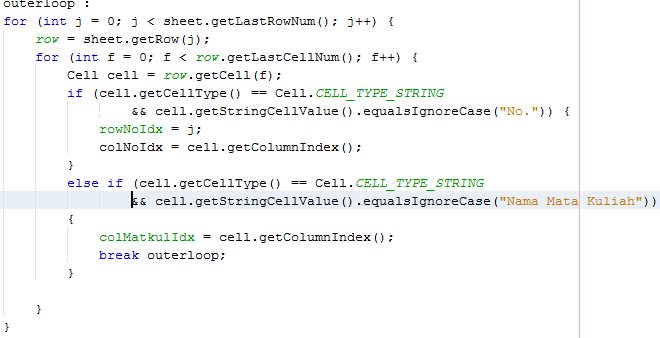
\includegraphics[scale=0.8]{Gambar/excelConverter1}
		\end{figure}
		\begin{figure}[H]
		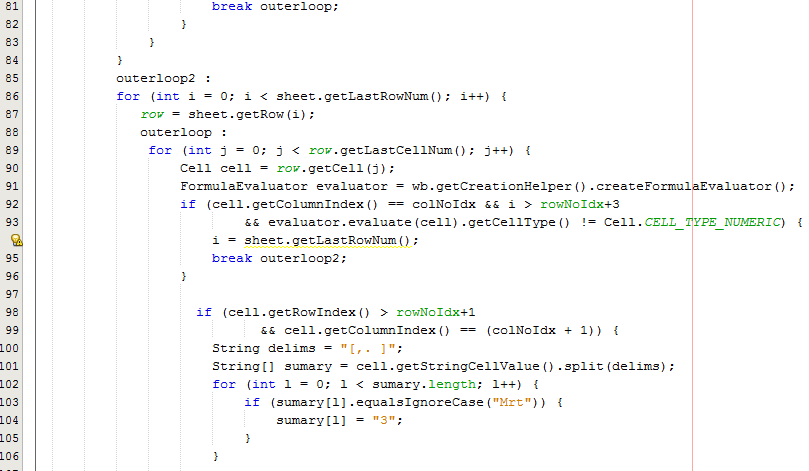
\includegraphics[scale=0.8]{Gambar/excelConverter2}
		\end{figure}
		\begin{figure}[H]
		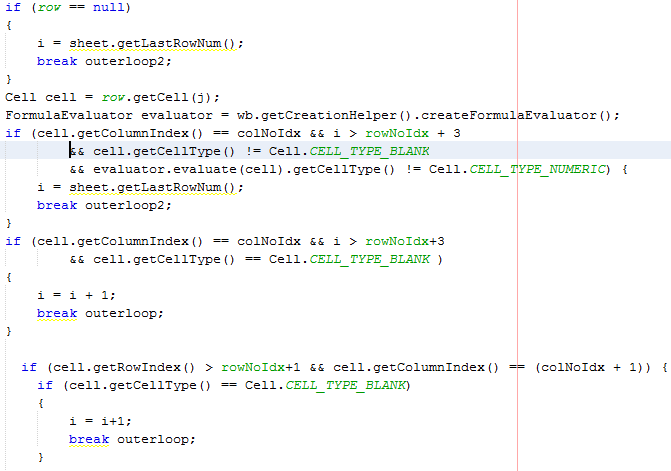
\includegraphics[scale=0.8]{Gambar/excelConverter3}
		\end{figure}
		\begin{figure}[H]
		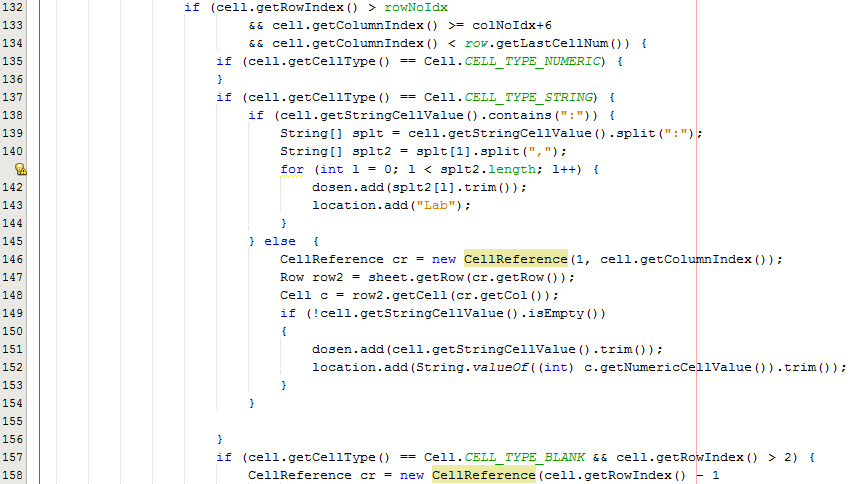
\includegraphics[scale=0.8]{Gambar/excelConverter4}
		\end{figure}
		\begin{figure}[H]
		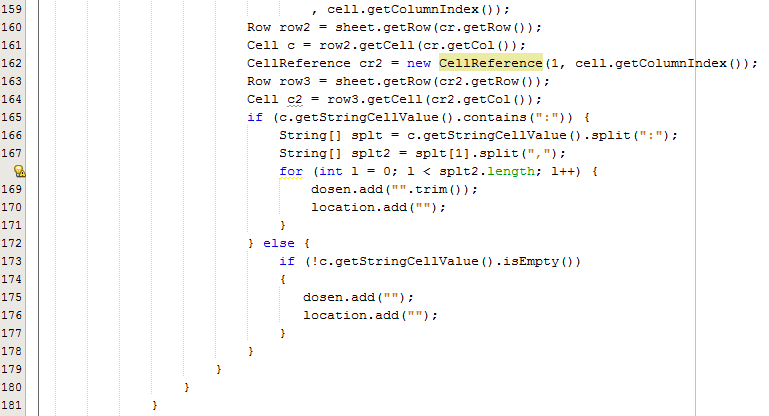
\includegraphics[scale=0.8]{Gambar/excelConverter5}
		\end{figure}
		\begin{figure}[H]
		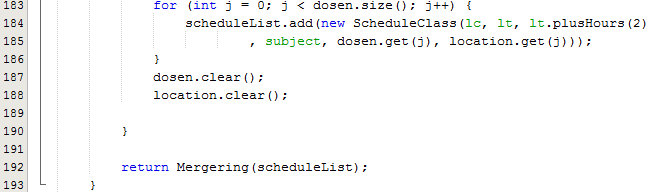
\includegraphics[scale=0.8]{Gambar/excelConverter6}
		\end{figure}
		\begin{figure}[H]
		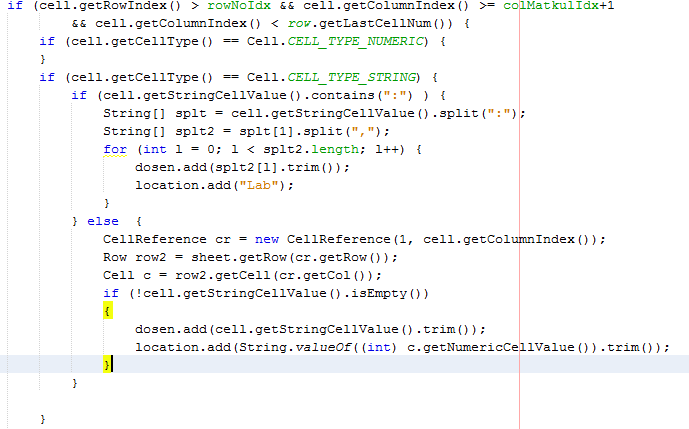
\includegraphics[scale=0.8]{Gambar/excelConverter7}
		\end{figure}
		\begin{figure}[H]
		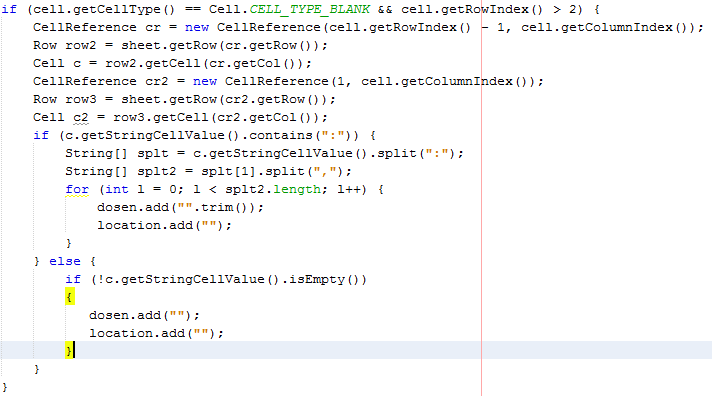
\includegraphics[scale=0.7]{Gambar/excelConverter8}
		\end{figure}
	\item Kode program untuk mengkonversi menjadi file iCalendar
		\begin{figure}[H]
		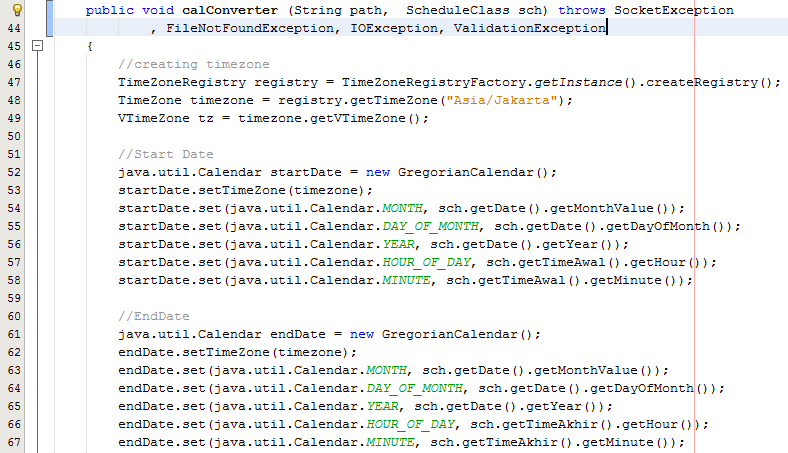
\includegraphics[scale=0.8]{Gambar/calConverter1}
		\end{figure}
		\begin{figure}[H]
		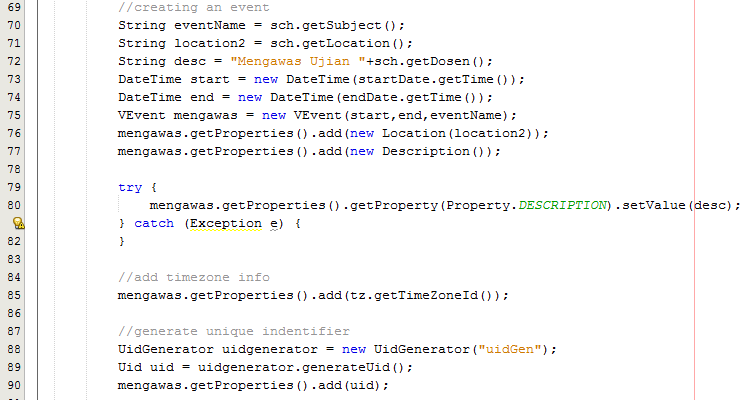
\includegraphics[scale=0.8]{Gambar/calConverter2}
		\end{figure}
		\begin{figure}[H]
		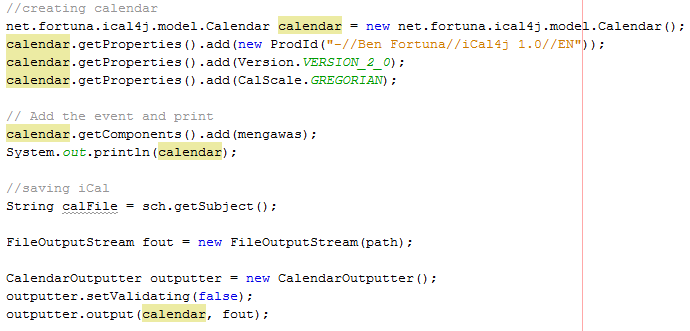
\includegraphics[scale=0.8]{Gambar/calConverter3}
		\end{figure}
	\item Kode program untuk menampilkan ke layar dan melakukan filter
		\begin{figure}[H]
		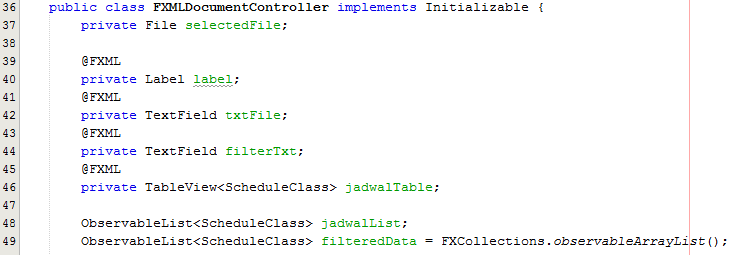
\includegraphics[scale=0.8]{Gambar/controller}
		\end{figure}
		\begin{figure}[H]
		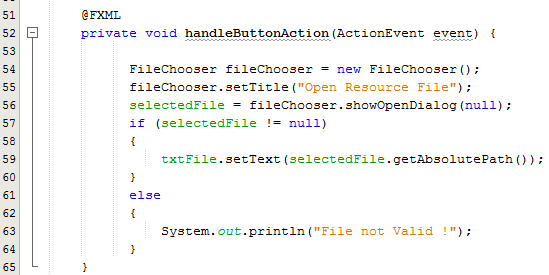
\includegraphics[scale=0.8]{Gambar/controller1}
		\end{figure}
		\begin{figure}[H]
		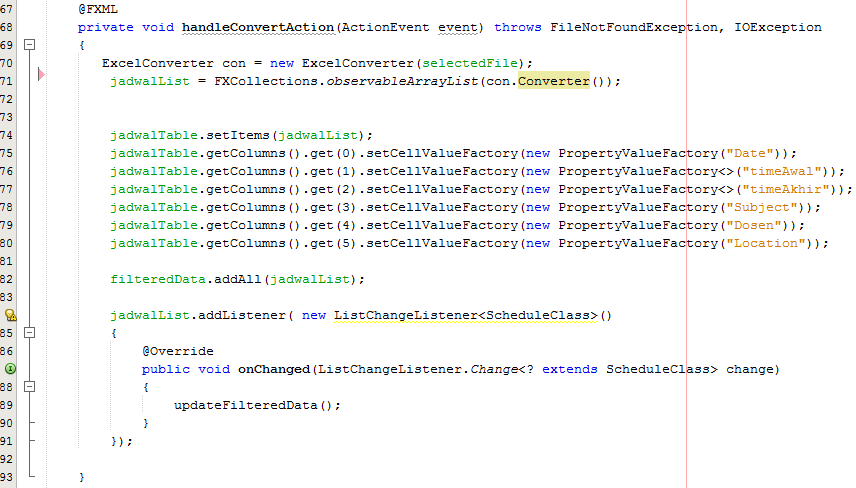
\includegraphics[scale=0.8]{Gambar/controller2}
		\end{figure}
		\begin{figure}[H]
		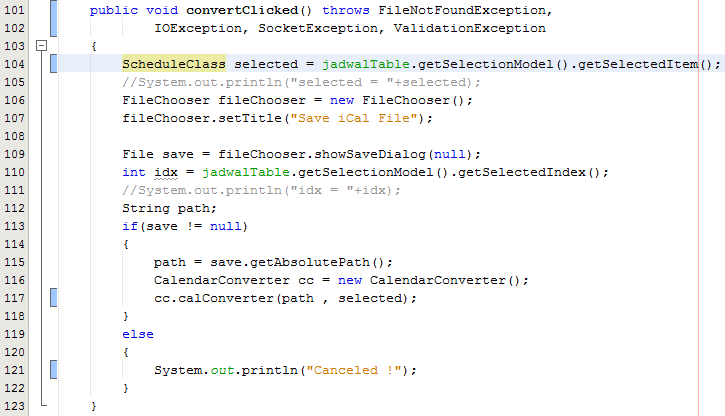
\includegraphics[scale=0.8]{Gambar/controller3}
		\end{figure}
		\begin{figure}[H]
		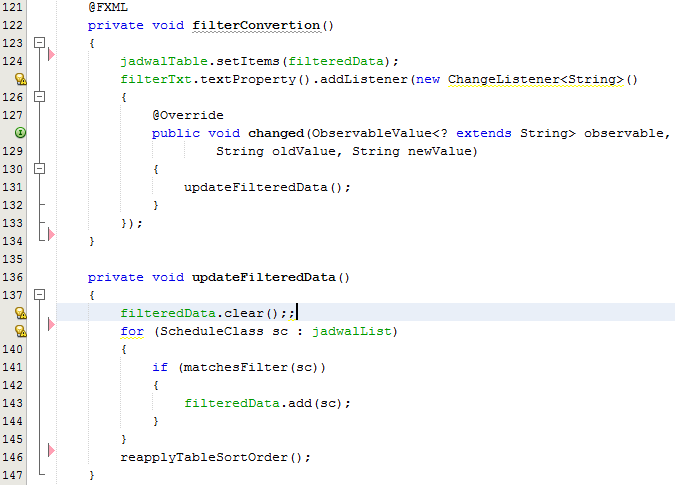
\includegraphics[scale=0.8]{Gambar/controller4}
		\end{figure}
		\begin{figure}[H]
		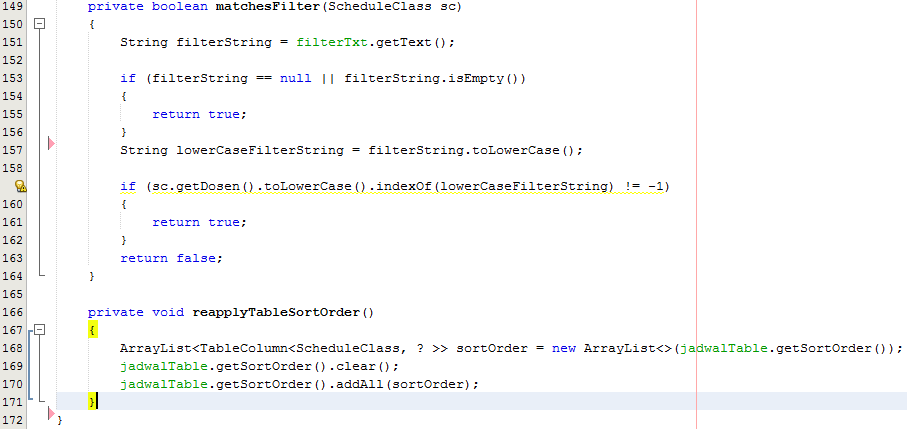
\includegraphics[scale=0.7]{Gambar/controller5}
		\end{figure}
\end{enumerate}

\section{Implementasi Antarmuka}
Berikut ini implementasi antarmuka dari perangkat lunak iCalendarConverter :
\begin{enumerate}
	\item Tampilan perangkat lunak iCalendarConverter
		\begin{figure}[H]
		\centering
		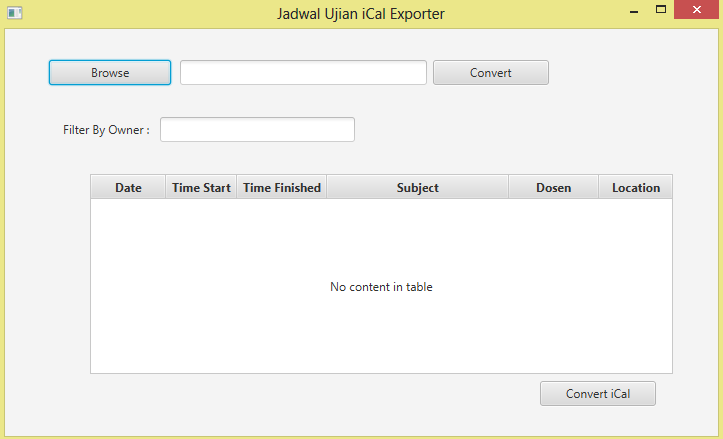
\includegraphics[scale=0.7]{Gambar/implementAntarmuka}
		\caption{Tampilan antarmuka perangkat lunak}
		\label{fig:implementAntarmuka}
		\end{figure}
	\item Tampilan Antarmuka ketika file excel jadwal mengawas telah dimasukan
		\begin{figure}[H]
		\centering
		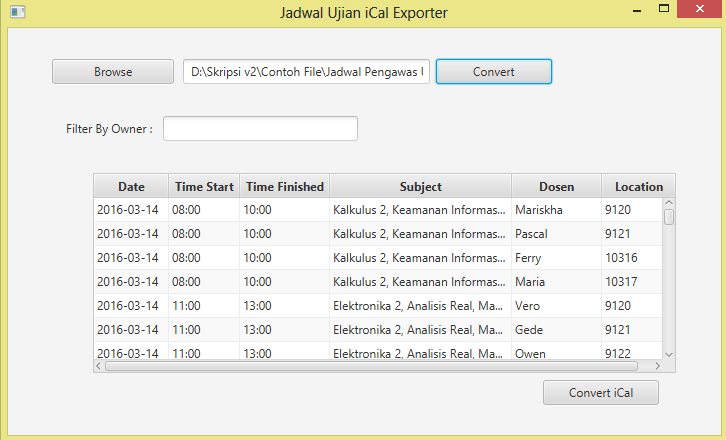
\includegraphics[scale=0.7]{Gambar/implementAntarmuka2}
		\caption{Tampilan antarmuka setelah file mengawas dimasukan}
		\label{fig:implementAntarmuka}
		\end{figure}
\end{enumerate}

\section{Pengujian}
Pada subbab ini akan dilakukan pengujian pada perangkat lunak untuk mengetahui apakah program dapat berjalan sesuai dengan apa yang di inginkan. Terdapat dua pengujian yaitu :
\begin{enumerate}
	\item Pengujian Fungsional.
	\item Pengujian Eksperimental.
\end{enumerate}

\subsection{Pengujian Fungsional}
Pada pengujian ini akan di uji mengenai fungsionalitas dari perangkat lunak ini, Berikut hasil pengujiannya : 
\begin{table}[H]
	\centering
		\caption{Tabel hasil pengujian fungsional}
		\label{tab:fungsional}
		\begin{tabular}{ | p{4cm} | p{4cm} | p{4cm} | c |}
			\hline
				Hal yang diuji & Hasil yang diharapkan & Hasil Pengujian & Status \\ \hline
				Browse file Excel & PL dapat melakukan browse file excel & PL dapat melakukan browse file excel & OK \\ \hline
				Path File Excel & PL dapat menangkap path file dari input & PL dapat menangkap path file dari input & OK \\ \hline
				Menampilkan Jadwal ke layar & PL menampilkan ke layar file excel yang telah dibaca  & PL menampilkan ke layar file excel yang telah dibaca & OK \\ \hline
				Konversi ke iCal & PL dapat mengkonversi jadwal kedalam iCalendar & PL dapat mengkonversi jadwal kedalam iCalendar & OK \\ \hline
				Filter nama dosen & PL dapat menampilkan nama dosen yang telah di filter & PL dapat menampilkan nama dosen yang telah di filter & OK \\ \hline
				Hasil Filter dapat dikonversi ke iCal & Hasil Filter pada PL dapat di konversikan kedalam iCal & Hasil Filter pada PL dapat di konversikan kedalam iCal & OK \\ \hline
				Import Google Calendar & Hasil konversi PL dapat di masukan kedalam Google Calendar & Hasil konversi PL dapat di masukan kedalam Google Calendar & OK \\ \hline
				Dapat dibuka di Outlook & Hasil konversi PL dapat di buka di Outlook & Hasil konversi PL dapat di buka di Outlook & OK \\ \hline
				Hasil filter dapat di import Google Calendar & Hasil filter konversi PL dapat di masukan kedalam Google Calendar & Hasil filter konversi PL dapat di masukan kedalam Google Calendar & OK \\ \hline
				Hasil filter Dapat dibuka di Outlook & Hasil filter konversi PL dapat di buka di Outlook & Hasil filter konversi PL dapat di buka di Outlook & OK \\ \hline
		\end{tabular}
\end{table}

Berikut ini adalah tampilan dari hasil pengujian yang telah dilakukan pada tabel ~\ref{tab:fungsional} :
\begin{enumerate}
	\item Browse File
		\begin{figure}[H]
		\centering
		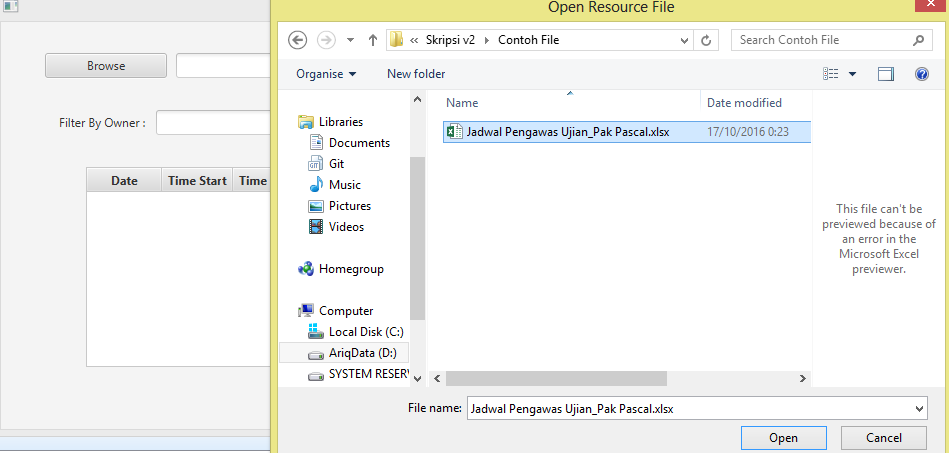
\includegraphics[scale=0.7]{Gambar/browseFile}
		\caption{Tampilan browse file excel mengawas ujian}
		\label{fig:browseFile}
		\end{figure}
	\item Path File Excel
		\begin{figure}[H]
		\centering
		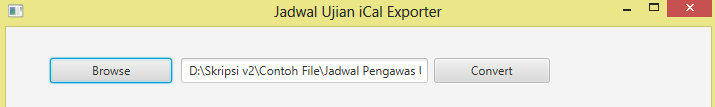
\includegraphics[scale=0.7]{Gambar/pathFile}
		\caption{Tampilan path file excel mengawas ujian}
		\label{fig:pathFile}
		\end{figure}
	\item Menampilkan jadwal ke layar
		\begin{figure}[H]
		\centering
		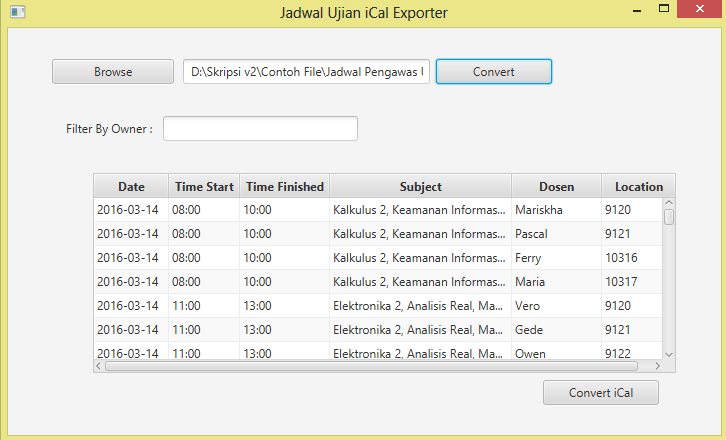
\includegraphics[scale=0.7]{Gambar/implementAntarmuka2}
		\caption{PL menampilkan jadwal ke layar}
		\label{fig:jadwalKeLayar}
		\end{figure}
	\item Konversi ke iCal
		\begin{figure}[H]
		\centering
		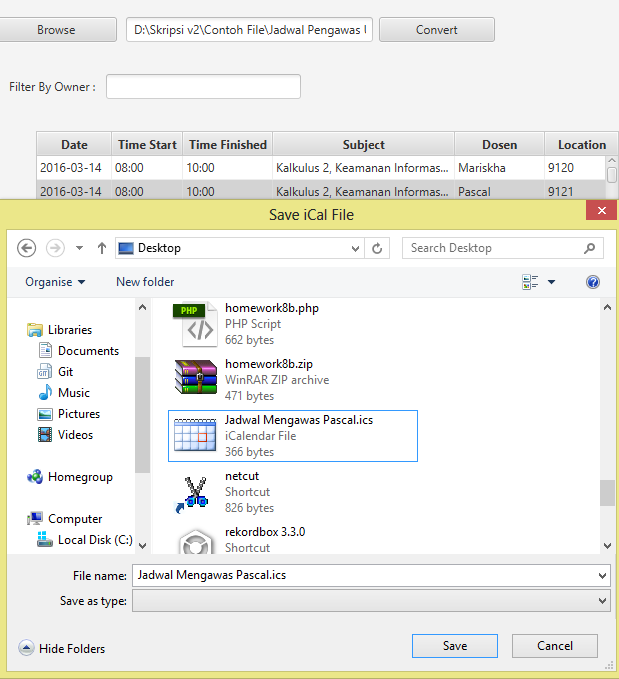
\includegraphics[scale=0.5]{Gambar/konversiiCal}
		\caption{PL mengkonversi jadwal ke format iCal}
		\label{fig:konversiiCal}
		\end{figure}
		
		\begin{figure}[H]
		\centering
		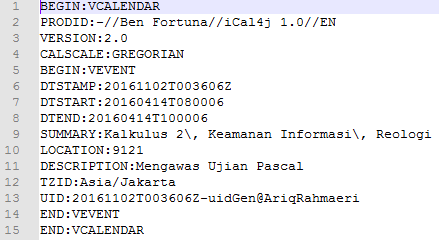
\includegraphics[scale=0.7]{Gambar/fileiCal}
		\caption{File iCal}
		\label{fig:fileiCal}
		\end{figure}
	\item Filter nama dosen
		\begin{figure}[H]
		\centering
		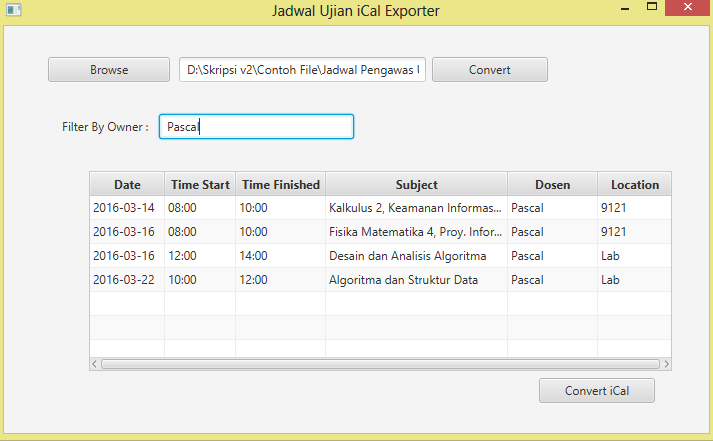
\includegraphics[scale=0.7]{Gambar/filterDosen}
		\caption{Hasil pengujian filter nama dosen}
		\label{fig:filterDosen}
		\end{figure}
	\item Convert hasil filter kedalam iCal
		\begin{figure}[H]
		\centering
		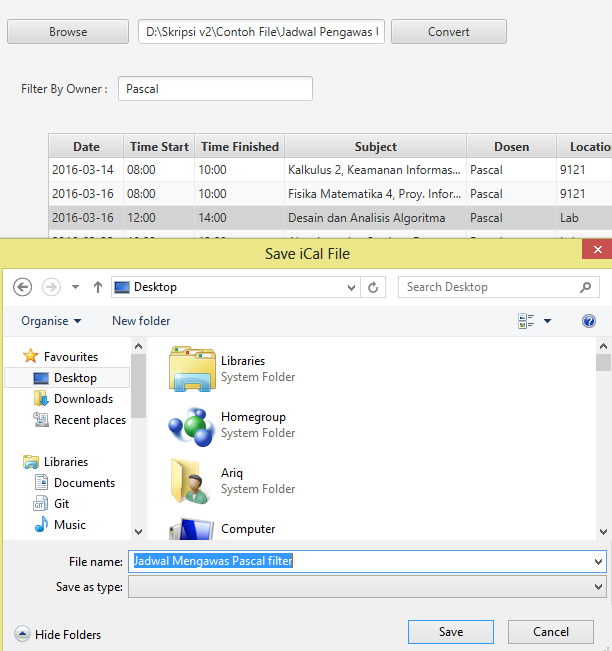
\includegraphics[scale=0.5]{Gambar/filterKonvertiCal}
		\caption{Hasil pengujian convert hasil filter kedalam iCal}
		\label{fig:filterKonvertiCal}
		\end{figure}
		
		\begin{figure}[H]
		\centering
		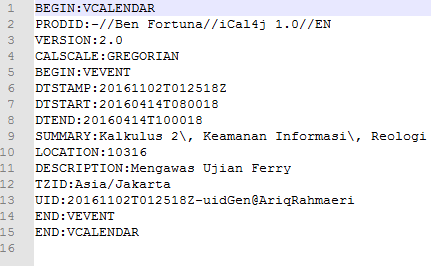
\includegraphics[scale=0.5]{Gambar/fileiCalFilter}
		\caption{File iCal Filter}
		\label{fig:fileiCalFilter}
		\end{figure}
	
	\item Import Google Calendar
		\begin{figure}[H]
		\centering
		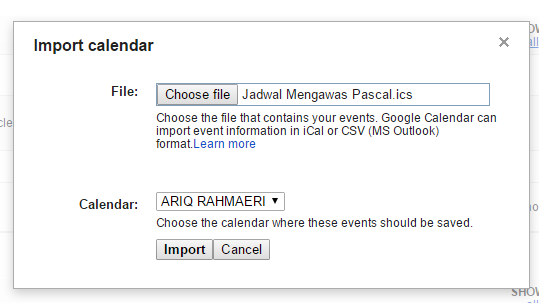
\includegraphics[scale=0.7]{Gambar/importGC}
		\caption{Hasil pengujian import kedalam Google Calendar}
		\label{fig:importGC}
		\end{figure}
		
		\begin{figure}[H]
		\centering
		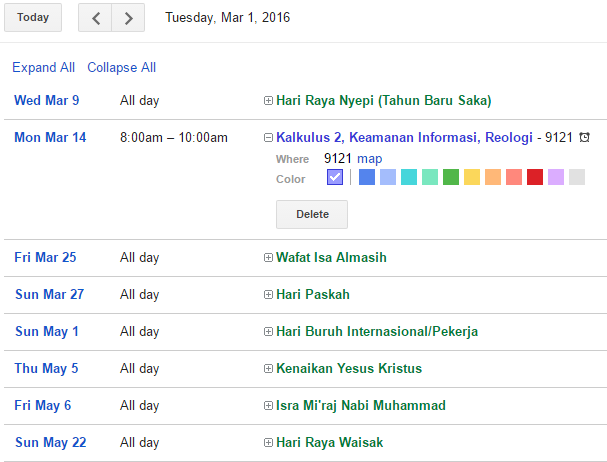
\includegraphics[scale=0.7]{Gambar/hasilGC}
		\caption{Hasil import ke Google Calendar}
		\label{fig:hasilGC}
		\end{figure}
		
		\begin{figure}[H]
		\centering
		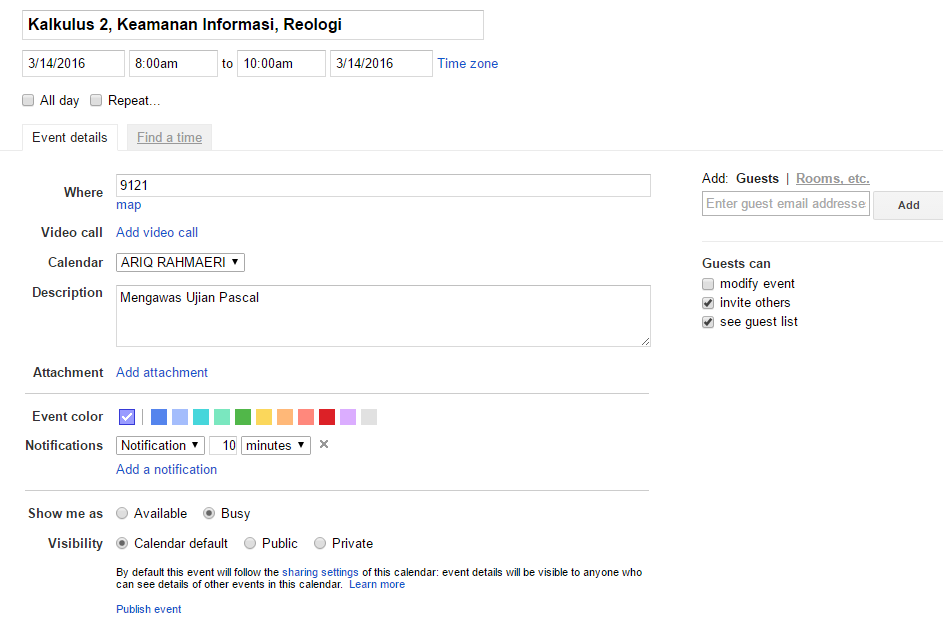
\includegraphics[scale=0.5]{Gambar/hasilGC2}
		\caption{Hasil import ke Google Calendar bagian 2 }
		\label{fig:hasilGC2}
		\end{figure}
		
		\item Buka di MS Outlook
			\begin{figure}[H]
			\centering
			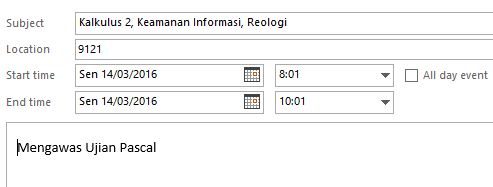
\includegraphics[scale=0.7]{Gambar/hasilOutlook}
			\caption{File hasil Konversi dapat dibuka di MS Outlook }
			\label{fig:hasilOutlook}
			\end{figure}
		
		\item Import hasil filter kedalam Google Calendar
			\begin{figure}[H]
			\centering
			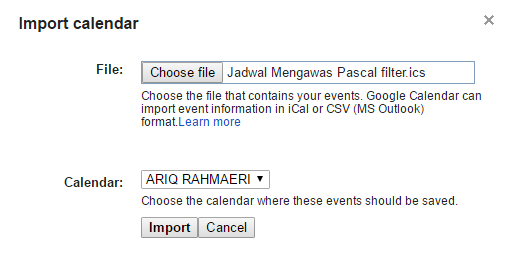
\includegraphics[scale=0.7]{Gambar/importGCFilter}
			\caption{Hasil pengujian import file yang di filter kedalam Google Calendar }
			\label{fig:importGCFilter}
			\end{figure}
			
			\begin{figure}[H]
			\centering
			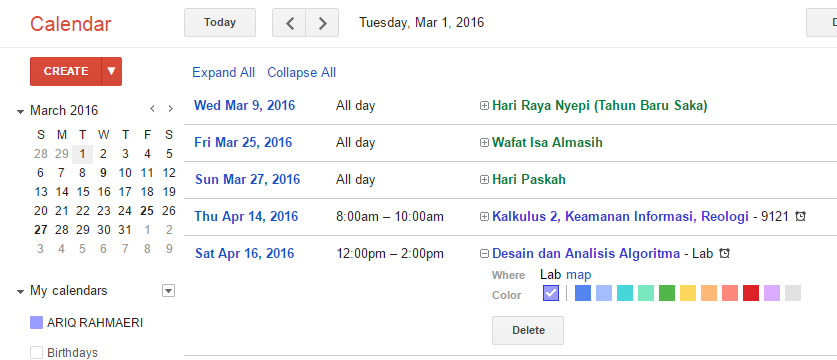
\includegraphics[scale=0.7]{Gambar/hasilGCFilter}
			\caption{Hasil import file yang di filter ke Google Calendar}
			\label{fig:hasilGCFilter}
			\end{figure}
			
			\begin{figure}[H]
			\centering
			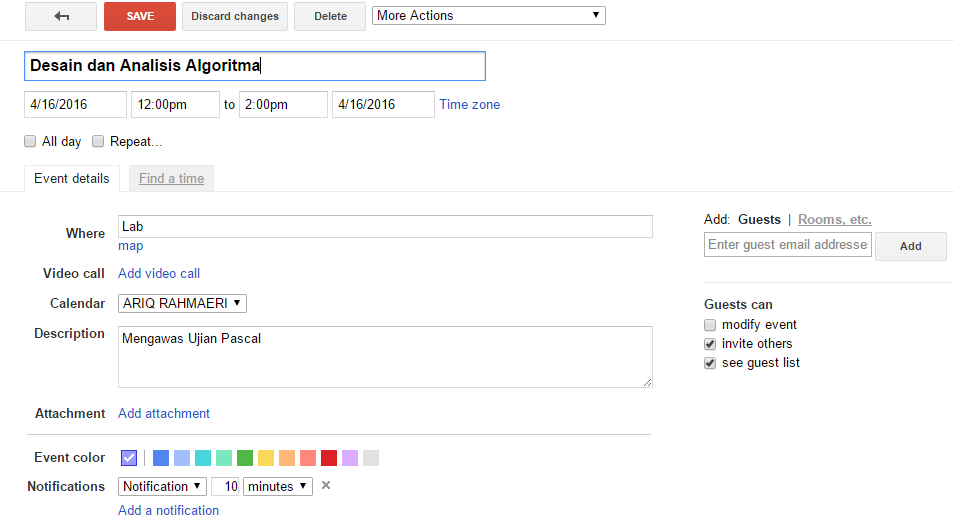
\includegraphics[scale=0.5]{Gambar/hasilGCFilter2}
			\caption{Hasil import file yang di filter ke Google Calendar bagian 2 }
			\label{fig:hasilGCFilter2}
			\end{figure}
			
		\item Buka hasil filter di MS Outlook
			\begin{figure}[H]
			\centering
			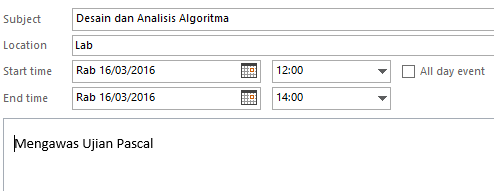
\includegraphics[scale=0.7]{Gambar/hasilOutlookFilter}
			\caption{File hasil filter dapat dibuka di MS Outlook }
			\label{fig:hasilOutlookFilter}
			\end{figure}
			
		
\end{enumerate} 

